\begin{multicols}{2}

\section{Game rules}

\subsection{Setting up the game}
\par Lay out the board and gather the players, dice and templates. Each coach will need their team, a dugout and a set of counters.
\par Each coach should place a Turn counter, a Score counter, and a Re-roll counter on the appropriate tracks.
\par Flip a coin; the winner chooses whether to kick or receive.

\begin{itemize}
\item The kicking team always sets up first.
\item A team must field eleven players and no more. If fewer than eleven players are available, field as many as you can.
\item At least three players must be set up next to the half way line, on the Line of Scrimmage. If fewer than three players are available you concede the match.
\item No more than two players may be set up in each wide zone.
\end{itemize}

\subsection{The kick-off}
\par After both teams have set up, the coach of the kicking team places the ball in any square in the opponent's half of the pitch (including the End Zone). Kicks are very inaccurate, so the ball will scatter. Before the scatter, the kicking player rolls on the kick-off table:

\medskip
\begin{tabularx}{\linewidth}{ | c | X | }
\hline
\textbf{2D6} & \textbf{Kick-Off Event} \\ 
\hline
2 & Each coach rolls 2D6; the high scorer's fans throw a rock at an opposing player. A tie means that both teams are affected. Select a player on the affected team(s) at random (only players on the field are eligible) and place them Stunned. \\
\hline
3 & The offence start their drive a fraction before the defence are ready; all of the players on the receiving team may move one square. This is a free move and may be made, ignoring tackle zones, into any adjacent empty square, including on the opposing half of the field. \\
\hline
4-5 & Shabby kick: add 3 to the D6 roll for the kick-off's scatter distance.\\
\hline
6-8 & No special event. \\
\hline
9-10 & Great kick: you may choose to change the D6 roll for the kick-off's scatter distance to a 1.
\\ \hline
11 & The kicking team shows instinctive defence; their coach may set the team up again, though the new setup must remain legal. The receiving team must remain in their existing positions. \\
\hline
12 & Each coach rolls 2D6, re-rolling any ties. The side with the highest score gets an extra re-roll this half. \\
\hline
\end{tabularx}
\medskip

\par Scatter the ball D6 squares, in a random direction determined by D8 (use the scatter template).
\begin{itemize}
\item If the ball lands in an empty square it will bounce one more square.
\item If it lands on a square occupied by a player, they must try to catch the ball.
\item If the ball scatters or bounces off the pitch, or into the kicking team's half, the receiving coach is awarded a Touchback and must give the ball to any player on their team. 
\end{itemize}
\par Once the kick-off has been taken you are ready to proceed to the first turn of the game.

\subsection{The sequence of play}
\par Blood Bowl is split into two halves of sixteen turns each (i.e. eight turns per coach). The game is played using a simple but strict sequence of play, with the receiving team taking a turn, followed by the kicking team, one after the other, until the end of the drive. A drive is defined as playing until a touchdown is scored or the half ends.

\subsection{Taking a turn}
\par Move the Turn counter one space along its track, then perform one Action with each player on the team.

\subsection{Player actions}
\par Each player on a team may perform one Action per turn.
\par You must declare which Action a player is going to take before carrying it out.
\par Players perform Actions one at a time. A player must finish their Action before another player can take one.
\par Actions other than Move and Block may only be declared once per turn.

\medskip
\begin{tabularx}{\linewidth}{ | X | }
\hline
\textbf{Move}: The player may move a number of squares equal to their MA. \\
\hline
\textbf{Block}: The player may make a single block against a player in an adjacent square. \\
\hline
\textbf{Blitz}: The player may move a number of squares equal to their MA. They may make one block at any point during the move, which costs one square of movement. \\
\hline
\textbf{Pass}: The player may move a number of squares equal to their MA. At the end of the move the player may pass the ball. \\
\hline
\textbf{Hand-off}: The player may move a number of squares equal to their MA. At the end of the move the player may hand off the ball. \\
\hline
\textbf{Foul}: The player may move a number of squares equal to their MA. At the end of the move the player may foul a Prone or Stunned opponent. \\
\hline
\end{tabularx}
\medskip

\subsection{Turnovers}
\par Normally, a turn ends when all of the players on the team have performed an Action, or the coach decides not to take any more Actions. However, certain events, called turnovers, cause a turn to end early:

\begin{itemize}
\item A player on the moving team is Knocked Down (though being injured by the crowd or being placed Prone is not a turnover unless the player is holding the ball)
\item A passed ball, or hand-off, is not caught by a member of the moving team before the ball comes to rest
\item A player from the moving team attempts to pick up the ball and fails
\item A pass attempt is fumbled (even if a player from that team catches the fumbled ball)
\item A player is ejected by the referee for a foul
\item A player attempts to throw a team-mate holding the ball and the ball carrier fails to land successfully (including due to a failed Always Hungry roll)
\end{itemize}

\par A coach that suffers a turnover is not allowed to take any further actions that turn, and any action being taken ends immediately even if it was only partially completed. Make armour and injury rolls for players that were knocked down, and if the ball was dropped then roll to see where it bounces to. Players who were stunned on previous turns should be turned face up, and then the opposing coach may start to take their turn.

\subsection{The Agility table}
\par The Agility table is used to work out the success or failure of a number of different Actions in Blood Bowl, including dodging, picking up the ball, and throwing or catching the ball. Each Action has its own set of modifiers.
\par A roll of 1 before modification always fails and a roll of 6 before modification always succeeds, for any Agility roll made during a game.

\medskip
\begingroup\setlength{\fboxsep}{0pt}\colorbox{lightBlue}{%
\begin{tabularx}{\linewidth}{ | X | c | c | c | c | c | c | }
\hline
\multicolumn{7}{| l |}{\textbf{Agility Table}} \\
\hline
AG & 1 & 2 & 3 & 4 & 5 & 6+ \\
\hline
Required D6 roll & 6+ & 5+ & 4+ & 3+ & 2+ & 1+ \\
\hline
\end{tabularx}%
}\endgroup
\medskip

\subsection{Movement}
\par A player may move a number of squares less than or equal to their Movement Allowance. Players may move in any direction or combination of directions, including diagonally, as long as they do not enter a square that holds another player.

\subsection{Tackle zones}
\par A standing player exerts individual tackle zones on each of the eight adjacent squares. A player who is Prone or Stunned does not exert any tackle zones.
\par In order to leave a square that is in one or more opposing tackle zones, a player must dodge. The player only has to dodge once in order to leave the square, no matter how many opposing tackles zones are on it.

\medskip
\begingroup\setlength{\fboxsep}{0pt}\colorbox{lightBlue}{%
\begin{tabularx}{\linewidth}{ | X | c | }
\hline
\multicolumn{2}{| l |}{\textbf{Dodge modifiers}} \\
\hline
Making a Dodge roll & +1 \\
\hline
Per opposing tackle zone on the square the player is dodging to & -1 \\
\hline
\end{tabularx}%
}\endgroup
\medskip

\par Make an agility roll with the appropriate modifiers for dodging. If it succeeds, the player may carry on moving (and dodging if required) until they have used up their full Movement Allowance. If it fails, the player is Knocked Down in the square they were dodging to (a roll must be made to see if they were injured) and the team suffers a turnover, ending their turn immediately.

\subsection{Going for it}
\par When a player takes any Action that involves moving, they may try to move one or two extra squares over and above their MA -- this is called "going for it".
\par Roll a D6 for the player after they have moved each extra square. On a roll of 1 the player trips and is Knocked Down in the square that they moved to; the opposing coach must roll to see if the player was injured. On any other roll the player moves without mishap. If the player is Knocked Down then their team suffers a turnover and their turn ends immediately.
\par A player that is taking a Blitz Action may "go for it" in order to make a block. Roll a D6 for the player after declaring that they will make the block. On a roll of 1 the player is Knocked Down as described above. On any other roll the player makes the block without mishap.

\subsection{Picking up the ball}
\par If a player moves into a square in which the ball is lying, they must attempt to pick it up. Players that move into the square with the ball at other times cannot pick up the ball, and instead it will bounce one square; this does not cause a turnover.

\medskip
\begingroup\setlength{\fboxsep}{0pt}\colorbox{lightBlue}{%
\begin{tabularx}{\linewidth}{ | X | c | }
\hline
\multicolumn{2}{| l |}{\textbf{Pick up modifiers}} \\
\hline
Picking up the ball & +1 \\
\hline
Per opposing tackle zone on the player & -1 \\
\hline
\end{tabularx}%
}\endgroup
\medskip

\par Make an agility roll with the modifiers for picking up the ball. If it succeeds, the player picks up the ball (place it on their base) and may carry on with their turn. If the roll fails, the player drops the ball, which will bounce one square; their team suffers a turnover and their turn ends immediately.

\subsection{Blocks}
\par Instead of moving, a player may throw a block at an opposing player in an adjacent square.  Players that are Prone may not perform a block,  and you may only make a block against a standing player. To see if a block works you will need to use the special Block dice.

\subsubsection{Blitzes}
\par Once per turn a player on the moving team is allowed to make a special Blitz move; the player may move and make a block. The block may be made at any point during the move, but costs one square of movement. The player may carry on moving after the effects of the block have been worked out, if they have any squares of movement left.

\subsubsection{Strength}
\par The number of dice that are rolled depends on the strengths of the two players involved. Obviously, if one player is stronger than the other they are more likely to knock down their opponent when they make a block:

\begin{itemize}
\item If the players' strengths are equal, one dice is rolled.
\item If one player is stronger, two dice are rolled and the stronger player may choose which one is used.
\item If one player is more than twice as strong, three dice are rolled and the stronger player may choose which is used.
\end{itemize}

\par Note that the coach of the player making the block always rolls the dice, but that the coach of the stronger player chooses which is used.

\subsubsection{Assisting a block}
\par After a block has been declared, team-mates of the attacker and the defender may give an assist. This allows two or more attackers to gang up on a single defender, or for one or more defenders to aid a companion against a block. Each of these extra players adds +1 to the Strength of the player that they are assisting. Assisting a block does not count as an Action, and a player can assist any number of blocks per turn. A player is allowed to make an assist even if they have moved or taken an Action.
\par The attacking coach must declare if any of their players will give an assist first, then the defending coach must add defensive assists with players from their team. In order to make an assist, the player:

\begin{itemize}
\item must be adjacent to the enemy player involved in the block.
\item must not be in the tackle zone of any other player from the opposing team.
\item must be standing.
\item must have their tackle zones.
\end{itemize}

\par The result of the block only affects the two players directly involved; any assisting players are not affected. Similarly, only the skills belonging to the two players directly involved in the block may be used on the result; skills belonging to assisting players cannot be taken advantage of by either side.

\subsubsection{Rolling the block dice}
\par To complete the block action, roll the appropriate number of dice and look up the result below:

\medskip

\begin{tabularx}{\linewidth}{  c  X  }
\raisebox{-.6\height}{
\includegraphics[width=3em]{ad}} & \textbf{Attacker Down}: The attacking player is Knocked Down. \\
\raisebox{-.6\height}{
\includegraphics[width=3em]{bd}} & \textbf{Both Down}: Both players are Knocked Down in their current squares, unless one or both of the players involved uses the Block skill; if a player uses the Block skill then they are not Knocked Down. \\
\raisebox{-.6\height}{
\includegraphics[width=3em]{pb}} & \textbf{Pushed Back}: The defending player is pushed back one square by the blocking player. The attacking player may follow up the defender. \\
\raisebox{-.6\height}{
\includegraphics[width=3em]{ds}} & \textbf{Defender Stumbles}: Unless the defender uses the Dodge skill they are pushed back and then Knocked Down. If they use the Dodge skill then they are only pushed back. The attacking player may follow up the defender. \\
\raisebox{-.6\height}{
\includegraphics[width=3em]{dd}} & \textbf{Defender Down}: The defending player is pushed back and then Knocked Down. The attacking player may follow up the defender. \\
\end{tabularx}
\medskip

\subsubsection{Push backs}
\par A player that is pushed back as a result of a block must be moved one square away from the player making the block; there are three eligible squares in each direction:
\medskip
\begin{center}
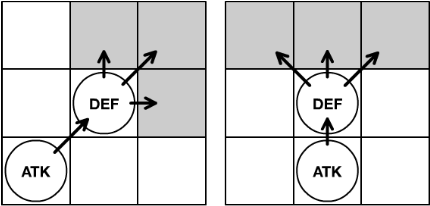
\includegraphics[width=0.6\columnwidth]{pushbacks}
\end{center}
\par The coach of the player who made the block may decide which square the player is moved to. The player must be pushed back into an empty square if possible. A square containing only the ball is considered empty, and a player pushed to it will cause the ball to bounce. If all such squares are occupied by other players, then the player is pushed into an occupied square, and the player that originally occupied the square is pushed back in turn. This secondary push back is treated exactly like a normal push back (Prone and Stunned players may be pushed in this manner as well). The coach of the moving team decides all push back directions for secondary push backs, unless the pushed player has a skill that overrides this.
\par Players must be pushed off the pitch if there are no eligible empty squares on the pitch. A player pushed off the pitch, even if Knocked Down, is beaten up only by the crowd and receives a roll on the Injury Table. The crowd does not have any injury modifying skills. Note that no Armour roll is made for a player that is pushed off the pitch: they are automatically injured. If a Stunned result is rolled on the Injury table the player should be placed in the Reserves box of the Dugout, and must remain there until the end of the drive. If the player who is holding the ball is pushed out of bounds, then they are beaten up by the fans, who are more than happy to throw the ball back into play! The throw-in template is centred on the last square the player was in before they were pushed off the pitch.

\subsubsection{Following up}
\par A player who has made a block is allowed to make a special follow up move and occupy the square vacated by the player that they have pushed back. The player's coach must decide whether to follow up before any other dice rolls are made. This move is free, and the player can ignore enemy tackle zones when they make the move (they do not have to dodge to enter the square). Players that are blitzing are allowed to make follow up moves, and the move does not cost them any more of their movement (they already paid a square in order to make the block).

\subsubsection{Knock downs}
\par A player that is Knocked Down should be placed on their side in the square, face up. The player may be injured. If the player who is Knocked Down comes from the moving team, this causes a turnover and the moving team's turn ends immediately.
\par Players that are Knocked Down or placed Prone for any reason should be placed face up on the pitch in the square they were in when they fell over. While Prone, the player loses their tackle zones and may do nothing until they stand up when they next take an Action.
\par A player who is carrying the ball and who is knocked down or placed Prone will drop the ball in the square where they fall. The dropped ball will bounce one square in a random direction after the player's armour/injury rolls are fully resolved.

\subsubsection{Injuries}
\par Unless the rules state otherwise, any player that is Knocked Down may be injured. The opposing coach rolls 2D6 in an attempt to beat the Knocked Down player's Armour value. If the roll succeeds, they roll on the Injury table to see what injury the player has suffered:

\medskip
\begin{tabularx}{\linewidth}{ | c | X | }
\hline
\textbf{2D6} & \textbf{Injury} \\
\hline
2-7 & Stunned: Leave the player on the pitch, but turn them face-down. All face-down players are turned face up at the end of their team's next turn (not the turn they are stunned), even if a turnover takes place. Once face-up they may stand up on any subsequent turn using the normal rules. Stunned players recover automatically at the end of the drive. \\
\hline
8-9 & KO: Take the player off the pitch and place them in the Dugout in the KO box. They will have a chance to recover at subsequent kick-offs. \\
\hline
10-12 & Casualty: Take the player off the pitch; they must miss the rest of the match. The opposing coach must roll on the casualty table to see if the player suffers any long-term effects. \\
\hline
\end{tabularx}
\medskip

\medskip
\begin{tabularx}{\linewidth}{ | c | X | }
\hline
\textbf{D6} & \textbf{Casualty} \\
\hline
1-3 & Badly Hurt: No long-term effect. \\
\hline
4 & Nasty Injury: Miss the next game. \\
\hline
5 & Niggling Injury: Miss the next game. Subsequent injury rolls against this player gain +1 per Niggling Injury. \\
\hline
6 & Dead \\
\hline
\end{tabularx}
\medskip

\par The coach of a player that suffers a casualty should make a note of its effect on their team roster.

\subsubsection{Substitutes}
\par You may not substitute fit players for injured players or players that have been sent off while a drive is in progress. The only time that you may add reserves is when you are setting up after a touchdown has been scored, or when setting up after half time.

\subsubsection{Standing up}
\par The only time a player can stand up is at the beginning of an Action, at a cost of three squares from their movement. If the player has fewer than three squares of movement, they must roll 4+ to stand up: if they stand up successfully, they may not move further squares unless they Go For It. Failure to stand successfully does not cause a turnover.
\par Players may stand up in an opposing player's tackle zone without having to make a Dodge roll. Note that a player who stands up may not take a Block Action.

\subsection{Passing}
\par Once per turn a player on the moving team is allowed to make a Pass Action. The player is allowed to make a normal move, and after they have completed the move they may throw the ball. Note that the player does not have to be holding the ball at the start of the Action; they could use their move to run over and pick up a ball on the ground and then throw it, for example.
\par Declare a Pass Action, move if desired, and then start the throw. It is perfectly acceptable to pre-measure the range to several players at any point during the throwing player's move before you declare the target of the pass. Once you have thrown the ball, you may not move the throwing player any farther that turn.

\begin{enumerate}
\item Declare the target of the pass and determine the appropriate range modifier.
\item Roll for any eligible interception.
\item Make an agility roll for the pass. If the pass is fumbled, suffer a turnover.
\item If the pass is inaccurate, scatter 3 times (to represent where the inaccurate pass lands, not the ball bouncing).
\item If the ball lands in a square with a player, roll to catch, otherwise bounce the ball once from the empty square the ball landed in.
\end{enumerate}

\subsubsection{Interceptions}
\par One player on the opposing team may attempt to intercept a thrown ball. Only one player can attempt an interception, no matter how many are eligible. To be able to make an interception, the player must:

\begin{itemize}
\item have the plastic ruler pass over at least part of the square they are standing in.
\item be closer to the thrower than the target square is.
\item be closer to the target square than the thrower is.
\item have their tackle zones.
\item The coach must declare that one of their players will try to intercept before the thrower rolls to see if they are on target.
\end{itemize}

\par Make an Agility roll with the modifiers for Interception.

\medskip
\begingroup\setlength{\fboxsep}{0pt}\colorbox{lightBlue}{%
\begin{tabularx}{\linewidth}{ | X | c | }
\hline
\multicolumn{2}{| l |}{\textbf{Interception modifiers}} \\
\hline
Attempting an interception & +1 \\
\hline
Per opposing tackle zone on the player & -1 \\
\hline
\end{tabularx}%
}\endgroup
\medskip

\par If it fails, the pass carries on as normal. If it succeeds, the player has caught the ball (place it on the player's base). A successful interception causes a turnover, and the moving team's turn ends immediately.

\subsubsection{The throw}

\medskip
\begingroup\setlength{\fboxsep}{0pt}\colorbox{lightBlue}{%
\begin{tabularx}{\linewidth}{ | X | c | }
\hline
\multicolumn{2}{| l |}{\textbf{Passing modifiers}} \\
\hline
Throwing a Quick Pass & +1 \\
\hline
Throwing a Short Pass & +0 \\
\hline
Throwing a Long Pass & -1 \\
\hline
Throwing a Long Bomb & -2 \\
\hline
Per opposing tackle zone on the player & -1 \\
\hline
\end{tabularx}%
}\endgroup
\medskip

\par Make an Agility roll with the modifiers for passing. If the roll for a pass is 1 or less before or after modification, the thrower has fumbled and dropped the ball. The ball bounces once from the thrower's square, and the moving team suffers a turnover and their turn ends immediately.
\par If the pass is not fumbled but the roll fails, the pass is inaccurate and scatters 3 times before landing. If the roll succeeds, the pass is accurate and lands in the target square.

\subsubsection{Catching the ball}
\par If the ball lands in a square occupied by a standing player on either team, then they must attempt to catch the ball. Prone and Stunned players may never attempt to catch the ball.

\medskip
\begingroup\setlength{\fboxsep}{0pt}\colorbox{lightBlue}{%
\begin{tabularx}{\linewidth}{ | X | c | }
\hline
\multicolumn{2}{| l |}{\textbf{Catching modifiers}} \\
\hline
Catching an accurate pass or hand-off & +1 \\
\hline
Catching a missed pass, kick-off, bouncing ball or throw-in & +0 \\
\hline
Per opposing tackle zone on the player & -1 \\
\hline
\end{tabularx}%
}\endgroup
\medskip

\par Make an Agility roll with the modifiers for catching. If the roll succeeds, the player has caught the ball (place it on the player's base). If it fails, then the player drops the ball, which will bounce.

\subsubsection{Bouncing balls}
\par The ball bounces if:

\begin{itemize}
\item it is dropped or not caught.
\item it lands on or bounces to a square with a Prone or Stunned player.
\item a player is pushed to or lands in its square.
\item it lands in an unoccupied square.
\end{itemize}

\par To find out where the ball bounces to, roll for scatter. If the ball bounces into an occupied square, then the player in the square must attempt to catch it. If it bounces into an empty square, it stops. If it bounces off the field, a Throw-in occurs.

\subsubsection{Throw-ins}
\par When a ball scatters or bounces off the pitch it is immediately thrown back in by the spectators. Use the Throw-in template to work out where the ball goes, using the last square the ball crossed before going off as a starting point. The ball is thrown 2D6 squares in a direction determined by D3. Throw-ins cannot be intercepted.

\subsubsection{Turnovers}
\par If a pass isn't caught by a player from the moving team, this causes a turnover and the moving team's turn ends. The turnover does not take place until the ball finally comes to rest. This means that if the ball misses the target but is still caught by a player from the moving team, then a turnover does not take place. The ball could even scatter or bounce out of bounds, be thrown back into an empty square, and as long as it is caught by a player from the moving team then the turnover is avoided.

\subsection{Handing off the ball}
\par A hand-off is where the ball is simply handed to another player, friend or foe, in an adjacent square. No dice roll is required to see if the player attempting the hand-off is successful -- it automatically hits the targeted player. However, the player that the ball is handed off to must roll to see if they catch the ball, treating it as an accurate pass.

\subsection{Fouls}
\par Normally, players that are Prone or Stunned cannot be attacked. However, one player per turn is allowed to take a Foul Action. This allows the player to move a number of squares equal to their MA and then make a foul against an opposing player who is Prone or Stunned and in an adjacent square.
\par The coach nominates the victim, and then makes an Armour roll for them.

\begin{itemize}
\item Any of the fouler's teammates that are adjacent to the victim must assist, each extra player adding 1 to the Armour roll.
\item Any of the victim's teammates that are adjacent to the fouler must assist, each extra player subtracting 1 from the Armour roll.
\item No player from either side may assist a foul if they are in the tackle zone of an opposing player (besides the fouler), do not have their tackle zones, or are not standing.
\end{itemize}

\par If the score beats the victim's Armour value then a roll is made on the Injury table to see what has happened to them.
\par Referees occasionally spot a player making a foul and send them off the pitch. To reflect this, if the Armour or Injury roll is doubles, the referee has spotted the foul, and the player taking the Foul Action is sent off for the rest of the match. In addition, their team suffers a turnover and their turn ends immediately. If the sent off player was holding the ball, the ball bounces from the square they were standing in when sent off.

\subsection{Re-rolls}
\par Re-rolls are very important in Blood Bowl. There are two types of re-rolls: team re-rolls and player re-rolls. In either case, a re-roll allows you to re-roll all the dice that produced any one result. No matter how many re-rolls you have, or what type they are, you may never re-roll a single dice roll more than once.

\subsubsection{Team re-rolls}
\par Team re-rolls represent how well trained a team is. A coach may use a team re-roll to re-roll any dice roll (other than Armour, Injury or Casualty rolls) made by a player on their team during their turn. A re-roll may be used even if the original roll was successful. The result of the new roll must be accepted in place of the first, even if it is worse. A coach may not use more than one team re-roll per turn, and may not use a re-roll to force the opposing coach to re-roll. Every time a coach uses up a team re-roll they must move their Re-roll counter down the track; when the counter reaches zero the coach may not use any more team re-rolls during the half. At half time the two teams get a chance to rest and recuperate, and so their team re-rolls are restored to their starting level.

\subsubsection{Player re-rolls}
\par Some players have skills that allow them to re-roll the dice under certain circumstances. A coach may use any number of player re-rolls in the same turn, and a single player may use a skill any number of times in the same match, though a single dice roll may not be re-rolled more than once.
\par You can't go back in time and use a skill or re-roll to affect an earlier Action. For example, if a player was blitzing, you couldn't have them throw a block, move a couple of squares, and then use their Pro skill to re-roll the block. The skill or re-roll must be used directly before or after the event it will affect or not at all.

\subsection{Scoring touchdowns}
\par You score a touchdown when one of your players is standing in your opponent's End Zone, while holding the ball, at the end of any of your players' Actions. As soon as this happens, play stops and the score marker is moved one space along the scoring track.
\par In some rare cases a team will score a touchdown in the opponent's turn. If one of your players is holding the ball in your opponent's End Zone at any point during your opponent's turn, your team scores a touchdown immediately, but you must move your Turn marker one space along the track.

\subsection{Restarting the match}
\par After a touchdown has been scored, and at the start of the second half, play is restarted and the match continues. Before the kick-off, each coach should roll a D6 for each KO'd player on their team. On a roll of 4+ the player is fit enough to return to play, but on any other result they must stay in the KO'd box in the Dugout.
\par Both coaches may then set up any fit players just as they did at the start of the game. When play is restarted after a touchdown, the scoring team is always the one to kick off. At the start of the second half, the kicking team is the one that did not kick off at the start of the first half.

\subsection{Winning the match}
\par The team with the most touchdowns at the end of the second half is the winner. If the match is tied it is declared a draw.
